This section describes the analysis methodology. We use boosted $Z\to\tauhad\taulep$ events to measure Monte Carlo correction factors for the tau identification algorithms in the high-$\pt$ region.

Different working points are defined for RNN score relative to the efficiency of selecting true $\tauhad$ candidates. When the efficiency of the working points is measured in data and simulation, a correction factor has to be derived and then applied to the simulation in order for the signal efficiency to agree between data and simulation \cite{ATLAS:2017mpa}. Because of the top quark mass, $t\bar{t}$ events are usually used as a source of high momentum taus for measuring correction factors on the high-$p_T$ bins. However, Lepton universality may not hold in W decays. For that reason our study is aimed to use boosted $Z\to\tauhad\taulep$ events for deriving and cross checking the simulation correction factors in the high-$p_T$ region.   
\subsection{Signal events}\label{signalevents}
For this study, we consider as signal events where one the taus decays hadronically and the other leptonically, either into an electron or a muon. Thus, our final states will include a $\tauhad$ candidate and a lepton $l=e,\mu$. The presence of the light lepton will be used as our tag. 
Generally, in $\Zll$ events, the taus are produced back to back and their $\pt$ spectrum falls sharply. In order to select boosted taus in the transverse plane we look for events where the opening angle in the transverse plane between the taus ($\Delta\phi(\tauhad,\taulep)$) is acute. A depiction of the topologies of our signal events is shown in Fig.\ref{Fig1}. For these events, the missing transverse momentum ($\met$) is assumed to come from the neutrinos produced in the decays of the tau leptons. Due to the fact that two neutrinos are produced in the leptonic decay mode we expect our events to have a larger $\met$ component along the $\taulep$ direction.
\begin{figure}[htbp]
	\centering
	\subfloat[]{\label{Fig1a}{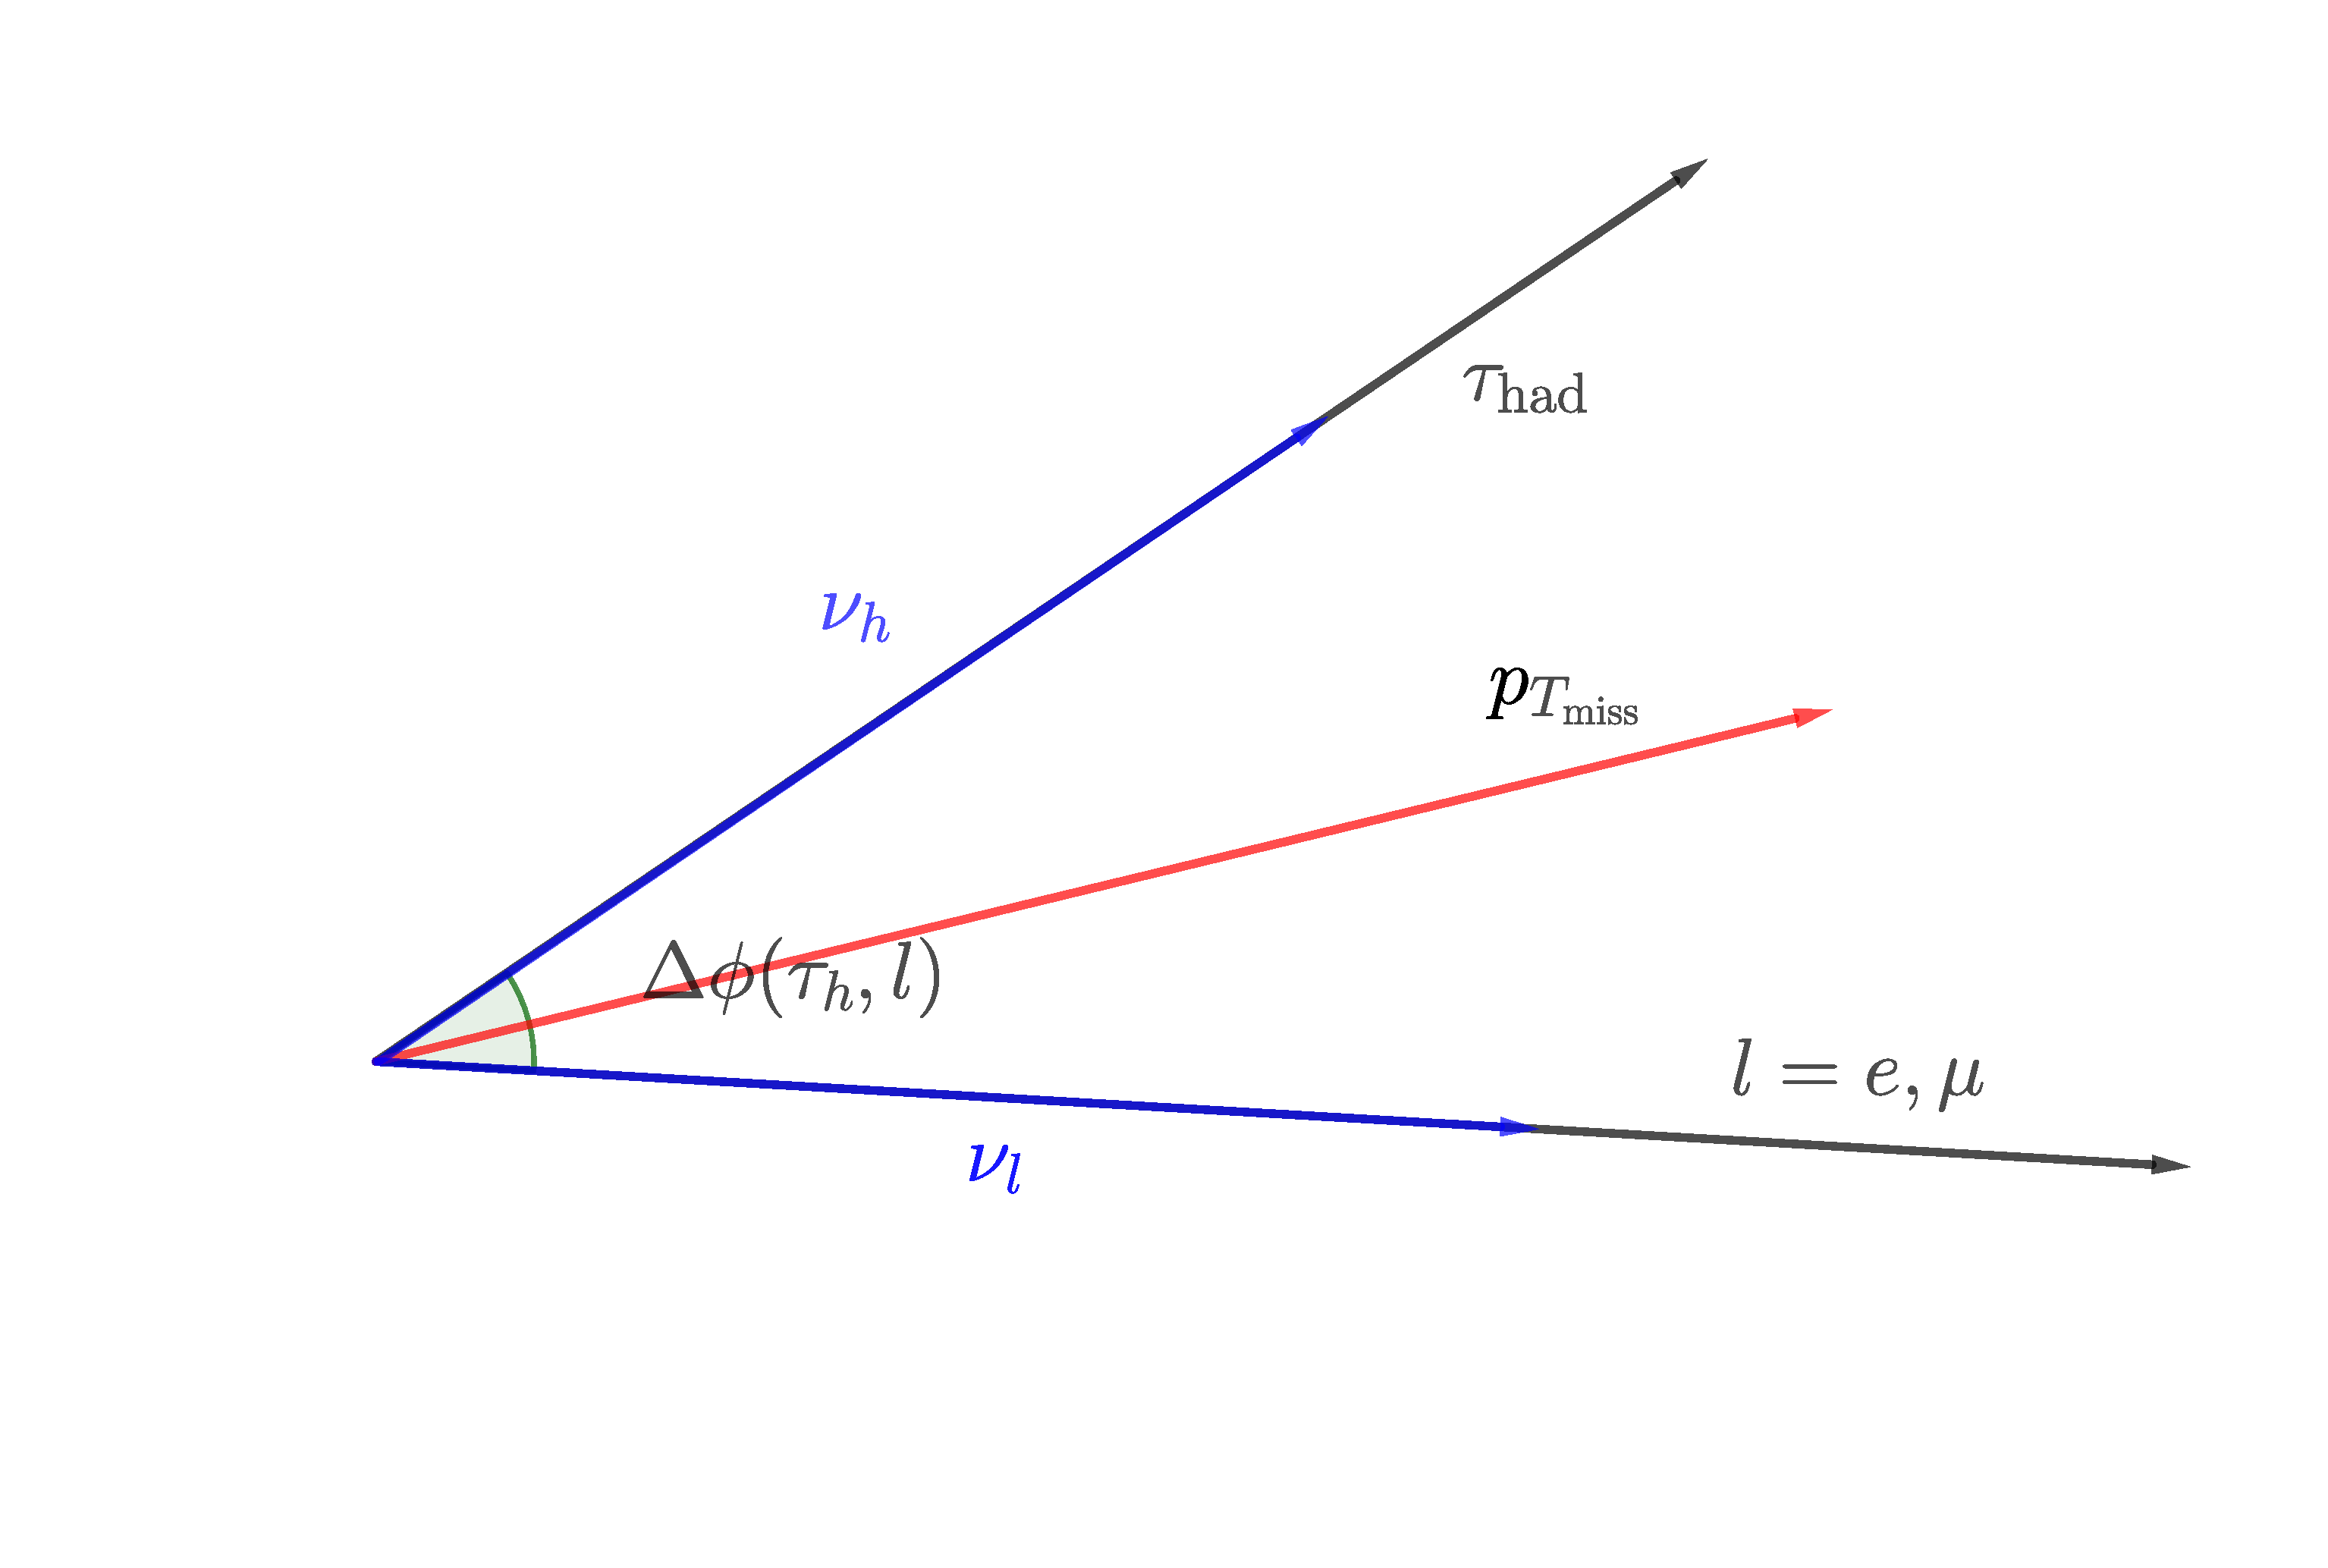
\includegraphics[width=0.49\textwidth]{Fig1a}}}\hfill
	\subfloat[]{\label{Fig1b}{\includegraphics[width=0.49\textwidth]{Fig1b}}}
	\caption{The two different types of topologies that define the signal events. On the left, when the missing energy is between the visible objects two neutrinos are assumed to be responsible for all the missing energy. On the right, only one neutrino is assumed to be flying on the direction of the visible object closest to the missing energy.}
	\label{Fig1}
\end{figure}
We classify our events in two types of topologies. First, events where the $\met$ is inside the opening angle between the visible objects. For this kind of events, we assume that the missing energy is due to a pair of neutrinos flying in the same direction as the visible objects. This is shown in Fig.\ref{Fig1a}. In this case, we solve the following equation to obtain the momentum of the neutrinos:
\begin{equation}
\vec{p}_{T_{\nu_l}}+\vec{p}_{\nu_h}=\vec{\met},
\end{equation}
given the following set of constraints (\textit{collinear approximation}):
\begin{align}
	\phi(\nu_l)&=\phi(l),
	\\
	\phi(\nu_h)&=\phi(\tauhad),
	\\
	\eta(\nu_l)&=\eta(l),
	\\
	\eta(\nu_h)&=\eta(\tauhad).
\end{align}
The second case, is when the $\met$ is pointing outside the angle formed by the visible objects, as is shown in Fig.\ref{Fig1b}. In this case, the assumption is that only one neutrino is responsible for the majority of the $\met$. We suppose it is flying in the direction of the visible object that is closest to the $\met$. We use the following equations to obtain the neutrino momentum:
\begin{align}
	p_{T_{\nu}}&=\met \cos(\Delta\phi(\tau_{\text{closer}},\met)),
	\\
	\phi(\nu)&=\phi(\tau_{\text{closer}}),
	\\
	\eta(\nu)&=\eta(\tau_{\text{closer}}),
\end{align} 
where $\tau_{closer}$ stands for the visible object closest to the direction of the $\met$.

We define a variable called $\Omega$ in order to classify our events in the already described topologies . First, we define:
\begin{equation}
\omega=\frac{\Delta\phi(\tau_{\text{closer}},\met)}{\Delta\phi(\tauhad,\taulep)},
\end{equation}
then,
\begin{itemize}
	\item when $\met$ is inside the opening angle between the visible objects but closer to $\tauhad$:
	\begin{equation}
	\Omega=\omega,
	\end{equation}
	\item when $\met$ is still inside, but closer to $\taulep$:
	\begin{equation}
	\Omega=1-\omega.
	\end{equation}
	\item If $\met$ is outside and closer to $\tauhad$:
	\begin{equation}
	\Omega=-\omega,
	\end{equation}
	\item and finally, if $\met$ is outside and closer to $\taulep$:
	\begin{equation}
	\Omega=\omega+1.
	\end{equation}
\end{itemize}
Thus, $\Omega$ is a continuous variable that give us information on the topology of the event. When $\met$ is inside the visible system it has values in the interval [0,1]. It is exactly 0 when $\met$ is in the $\tauhad$ direction and 1 when $\met$ is in the $\taulep$ direction. $\Omega$ has negative values when $\met$ is outside and closer to the $\tauhad$ candidate and has positive and values greater than 1 when is outside and closer to the $\taulep$. A diagram describing the $\Omega$ values is shown in Fig.\ref{Fig2}.
\begin{figure}[htbp]
	\centering
	\includegraphics[width=0.5\textwidth]{Fig2.png}
	\caption{Graphical representation of the different values of $\Omega$ depending on the region where the $\met$ is located in the event.}
	\label{Fig2}
\end{figure}
As we will see later, the event classification into these different types of topologies will allow us to reconstruct and exploit kinematical variables as the invariant mass of the di-tau system, the Z boson transverse momentum ($Z\pt$) and the angular distribution of the objects in the event.

\subsection{Scale Factors Calculation}
Conventionally, the correction or scale factors (SFs), are defined as the ratio of the efficiency in data and simulation of a $\tauhad$ candidate to pass a certain level of identification. This method makes the measurement sensitive not only to the uncertainties coming from the tau reconstruction but to the light lepton trigger, reconstruction and identification. Additionally, $\POWPY$ and $\SHERPA$ simulations give different predictions for the $Z\pt$. Consequently, differences in the kinematics of the reconstructed objects also affect the measurement.

Therefore, an alternative approach has been taken. First, the ratio of observed signal events to predicted events in simulation for $Z\to\tauhad\taulep$ is defined as:
\begin{equation}
	C_{X}=\frac{\NData}{\NMC}.
\end{equation}
Where X could be any of the tau-ID working points, 